
\newglossaryentry{X}
{
  type=differential-privacy,
  name={$\ensuremath{X} $},
  description={Set of locations for a user. ($R^2$)},
}
\newglossaryentry{Z}
{
  type=differential-privacy,
  name={$\ensuremath{Z} $},
  description={For every $x \in X$ a perturbed location $z \in Z$ is reported.},
}
\newglossaryentry{K}
{
  type=differential-privacy,
  name={$K(x)(Z)$},
  description={Randomization method for $x \in X$ and output $z \in Z$.},
}
\newglossaryentry{Epsilon}
{
  type=differential-privacy,
  name={$\ensuremath{\epsilon} $},
  description={The privacy budget $\epsilon$ determines the amount of noise that is added.
    },
}
\newglossaryentry{Pr}{
  type=differential-privacy,
  name={$Pr(K(x_i) \in (Z))$},
  description={Probability of reporting $x \in X$ for $z \in Z$}
}


\section{Differential privacy} \label{section:dp}
\todo[inline]{Explain general notion of privacy}
\glsaddall
\leading{10pt}
\printglossary[type=differential-privacy, nonumberlist]
\begin{figure}[h]
  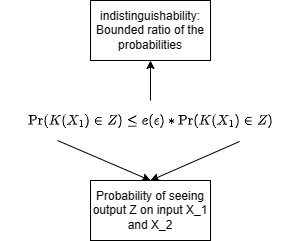
\includegraphics{TheorethicalFramework/Differential privacy/master-thesis-Differential privacy illustration.png}
  \caption{Randomization function $K$ gives $\epsilon$-differential privacy for all elements in $D_1$ and $D_2$ if they differ at most one element. \citep{dwork_differential_2006}}
  \label{fig:definition-dp}
\end{figure}
The privacy budget $\epsilon$ determines the amount of noise that is added.
\subsection{Laplace algorithm}
One way to achieve $\epsilon$-DP is using sampling noise from the Laplace or Gaussian distributions.
\todo[inline]{Explain gaussian / laplace distributions}
The noise is then based on the sensitivity of a function $f$.
This is the maximal possible change when adding or removing a single record \citep{friedman_data_2010, dwork_differential_2006}.
\begin{equation}
  \Delta f = max_{D_1, D_2} ||f(D_1) - f(D_2)||
\end{equation}
% This means, that if the sensitivity is low, the noise is as well.
% The metric is combined with the privacy budget $\epsilon$ to control the noise that is being added by a mechanism like Laplace \citep{friedman_data_2010}.
\todo[inline]{Explain differential privacy implementation with La place distribution}



\subsection{Local differential privacy}
\subsection{Geo-indistinguishability}
\subsection{Attacks on privacy}
\textbf{Membership inference attacks:}
An attack model that plays a big role in machine learning is a membership inference attack.
With this attack, an adversary attempts to infer the original data point $x \in X$ from a given data point $z \in Z$.
The adversary has access to a point $z$, the size of the dataset $|Z|$ and a distribution D where $Z$ was drawn from \citep{yeom_privacy_2018}.
These attacks depend on the adversarial knowledge, which can be divided into white-box and black-box MIA's \citep{hu_membership_2022}.
\begin{enumerate}
  \item \textbf{White-box}: The attacker has all the data that is needed. Including target model parameters, the training dataset and even the architecture \citep{hu_membership_2022}.
  \item \textbf{Black-box}: The attacker has a limited amount of information, like training data distribution and the trained model \citep{hu_membership_2022}.
\end{enumerate}

An approach called \textit{Binary classifier membership inference attacks} is used to separate members from non-members. \citep{hu_membership_2022}.
This method evolves around the attacker generating a shadow model, with as goal to overfit \citep{shokri_membership_2017}.
If the data is fed with real data the score is higher than similar data, which means the real data can be inferred \citep{shokri_membership_2017,jayaraman_evaluating_nodate}
A white-box setting requires a lot of adversarial knowledge for training the shadow models.
The black-box settings only take the prediction as input and decide if it is a (non-) member \citep{hu_membership_2022}.
An unsupervised black-box MIA was introduced by Peng et al. and only considers that the attacker has access to the already trained model.
They rescale the probabilities first using temperature scaling, to compensate for models that are overconfident \citep{peng_unsupervised_nodate}.
So instead of having a probability between two classes with for example 99\% against 1\% it will be more evenly distributed based on the training data.
They then proceed in clustering the probabilities into two clusters using K-Means and label the higher confidence scores as members.

The above attacks do rely on the model to also provide the confidence or probabilities of the predictions.
This is often not the case for the practical appliance of a model, and therefore Choquette-Choo et al. introduced a label-only attack.
While the existing models exploit the probability output for MIA, they solely rely on labels.
For this, they make use of the "HopSkipJump" attack; a so-called decision-based attack \citep{chen_hopskipjumpattack_2020}.
Choquette-Choo et al. consider a more semi-black-box approach, for which the attacker still requires access to a subset of the original training data and the trained model.
Another paper that also uses "HopSkipJump" requires only the trained model and achieves higher accuracy by using an approach with random data \citep{li_membership_2021}.

Another take on this is prediction and confidence-based MIA which are both proposed by \citep{yeom_privacy_2018}.
They assume that an attacker knows the standard error and has access to the perturbation dataset.
The algorithm is be-able to extract the truth label by minimizing the loss. \newline

To conclude on this, there are many methods for MIA and in that regard; the unsupervised methods look the most promising.
They require less setup and there is plenty of black-box approaches that score between 70\% and 80\% success rates.
For our use case, however, it is harder to establish an MIA; as we focus mainly on clustering.
Anyhow, it is possible if we consider a semi-supervised approach where we consider the cluster labels as ground truth (\ref{})
Differential privacy is proposed as a way of solving the inference attack for both white-box and black-box \citep{hu_membership_2022}.
However, it is hard to find a way to protect privacy and utility as well, so it depends heavily on the privacy budget.
In addition, it is hard to establish a member-inference attack on clustering as it requires a semi-supervised approach to be effective, as MIA requires classification \ref{fig:unsupervised-mia-attack}.


\textbf{Reconstruction attacks:}
Another attack that is a threat, especially to differential privacy is a reconstruction attack.
This attack is also more known as the attribute inference attack and is more focused on the data itself than machine learning models \citep{rigaki_survey_2021}. \newline
\textbf{Model extraction attacks:}
The final attack that is considered, is the model extraction attack.
This attack consists of the attacker being able to reconstruct and gather information about the original model.

% Jayaraman et al. evaluate inference attacks and differential privacy and express a metric called "privacy leakage"  \citep{jayaraman_evaluating_nodate}.


\begin{figure}
  \label{fig:unsupervised-mia-attack}
  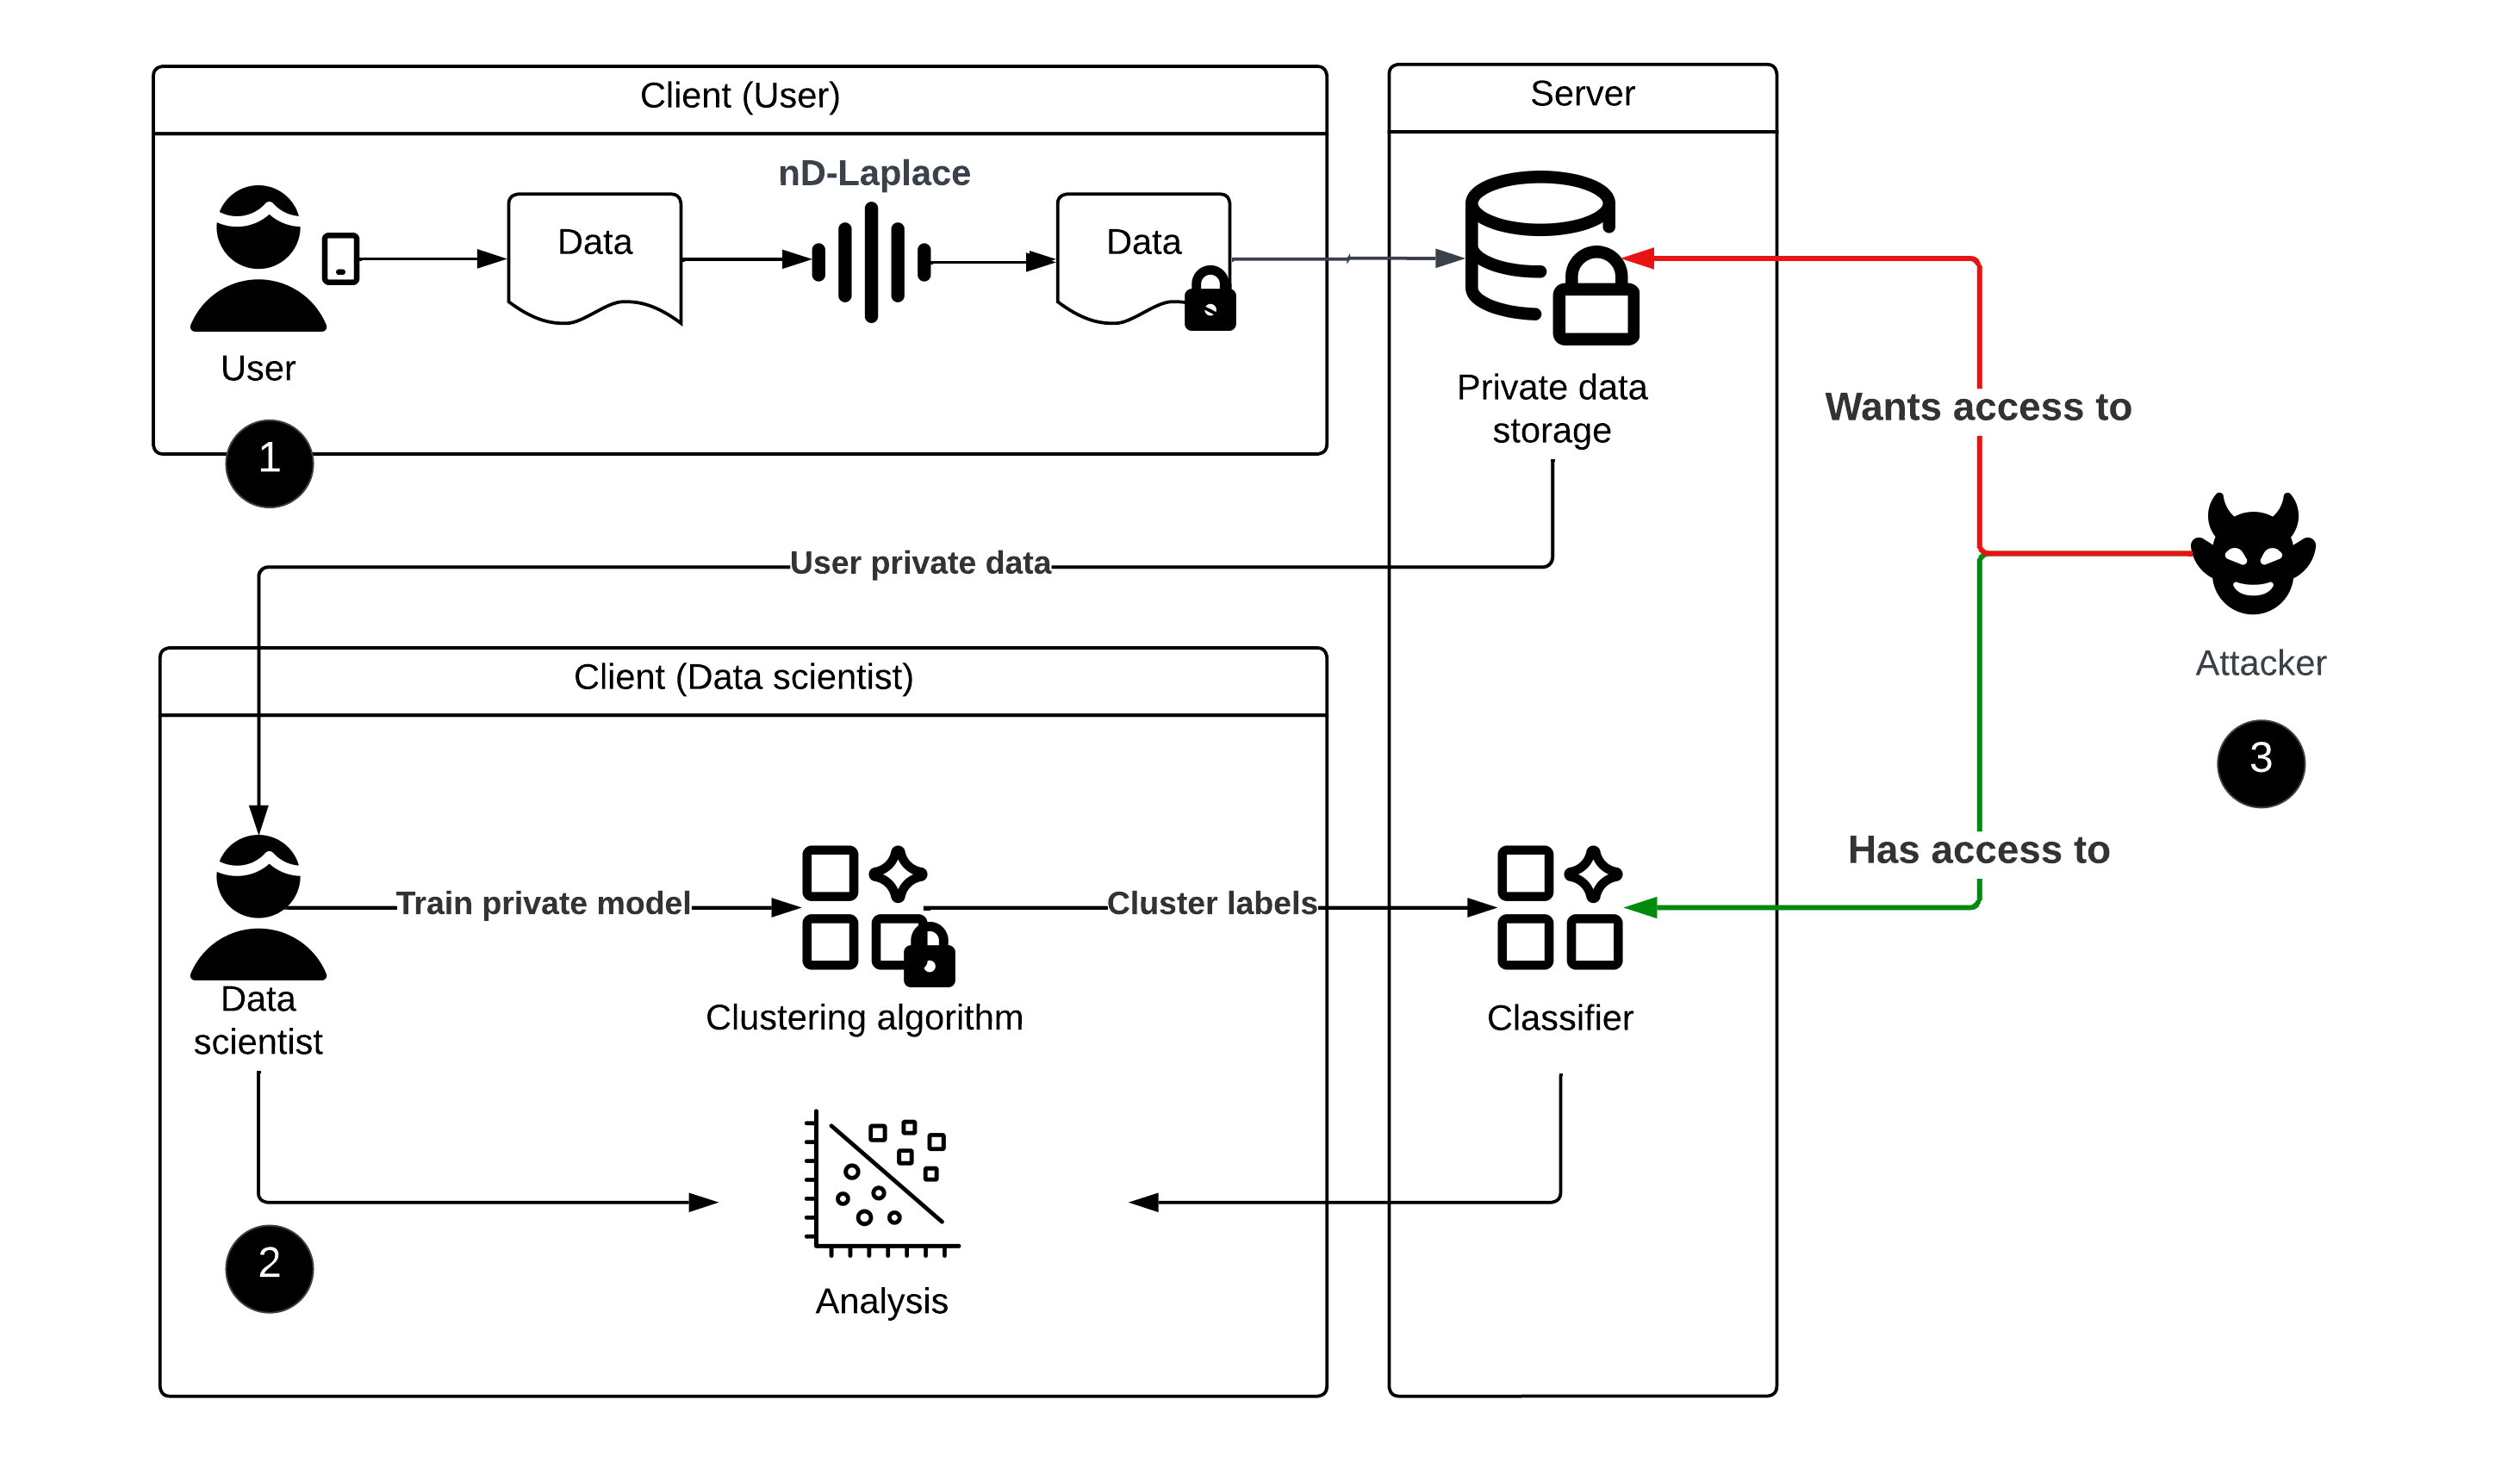
\includegraphics[width=1.0\textwidth]{TheorethicalFramework/Differential privacy/master-thesis-MIA.png}
  \caption{Semi-supervised membership inference attack considering a black-box approach \citep{chen_hopskipjumpattack_2020,li_membership_2021}}
\end{figure}

%The above attacks mainly target the clustering method after they have been trained. 
%$Various attacks are more focused on data, like 
\subsection{Evaluation methods} \label{theory:evaluation-dp}
It is possible to evaluate and measure the impact of the noise between two distributions by calculating the error between the non-private and private data \citep{del_rey_comprehensive_2020-1}.
Two metrics that are proposed by the same study are Mean Squared Error (MSE) and Mean Average Error (MAE).
These metrics can be used to calculate the error between $X$ and the perturbed dataset $Z$. \newline

Just as it is possible to measure the utility, this can also be done with privacy.
When performing a privacy algorithm, it can be proven whether a method meets the privacy requirements.
These are metrics such as $\epsilon$-differential-privacy (\ref{fig:definition-dp}) and $\epsilon$-geo-indistinguishability (see next chapter \ref{algo:2d-geo-indistinguishability}).
Although these methods give an idea of privacy, it can only be "yes" or "no".
Furthermore, it can give a distorted image, since a chance of 70\% also gives a "yes" according to the definition of geo-indistinguishability \citep{oya_is_2017}.
In other words, to gain more insight into the amount of privacy (such as with MSE or MAE), other metrics are needed.

For this reason, Oya et al. introduced a metric for geo-indistinguishability that makes it possible to give percentages in their study \citep{oya_is_2017}:
As an example, an adversary is given that guesses between two locations: $x \in X$ and  $x' \in X$.
\begin{equation}
  p_e (x, x', z) \leq p^*_e = \frac{1}{1 + e^{e * d(x, x')}}
  \label{eq:geo-as-an-error}
\end{equation}
Where privacy level $p^*_e$ is the lower bound of the probability of an adversary guessing correctly.
The method is called $\epsilon$-geo-indistinguishability as error.
Based on this metric, it can be calculated that an adversary has an average of 90\% chance to guess a location correctly.
In that case, the algorithm would be $\epsilon$-geo-indistinguishability, but in practice not.